\chapter{Neurophysiologie}
\label{Chapitre: Neurophysiologie}
\thispagestyle{fancy}

Le système nerveux est un ensemble de structures complexes permettant à un animal d'interagir avec les différentes parties de son corps, ainsi qu'avec son environnement extérieur. Celui de l'Homme est composé de deux structures  :

\smallbreak
\begin{itemize}
	\item Le Système Nerveux Central (SNC). Centre de décision, Il est composé du cerveau et de la moelle épinière. 
	\smallbreak
	\item Le Système Nerveux Périphérique (SNP). Il est constitué de nerfs et de ganglions, qui ont pour rôle de connecter les muscles ainsi que les structures éfferentes au Système Nerveux Central (SNC). Il est également composé de centres de décision autonomes, on parle alors de système nerveux autonomes (exemple : le système nerveux sympathique gérant de nombreuses activités dites inconscientes, comme le rythme cardiaque). 
\end{itemize}
\smallbreak
Nous nous intéressons plus particulièrement au SNC, les interfaces cerveau-ordinateur étant effectuées à partir de l'étude des signaux produits par le cerveau. 

\section {Cartographie du cerveau humain}
\label{Section: 2.Cartographie du cerveau humain}

Le cerveau humain est constitué de 2 éléments : l'aire corticale (elle même composée des lobes externes) et une partie interne, (composée des lobes limbiques) \cite{mcGill}. 

\subsection{Lobes externes}
\label{Subsection: 2.Lobes externes}
Le cortex cérébral est constitué de deux hémisphères : un hémisphère droit et un hémisphère gauche (souvent appelé cerveau droit et cerveau gauche) contrôlant l’ensemble de nos fonctions cognitives : mouvements volontaires, pensée, mémoire, etc. D’une manière générale, l’hémisphère droit commande le côté gauche du corps et inversement. (Figure \ref{test})

\begin{figure}[h]
	\centering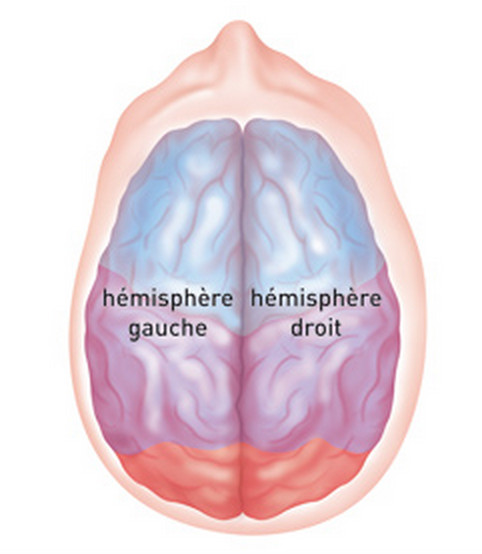
\includegraphics[width=5cm]{images/brainMap2.png}
	\caption[Les deux hémisphères du cerveau]{Les deux hémisphères du cerveau.\\Source : http://intelligences.livehost.fr/}
	\label{test}
\end{figure}

Chaque hémisphère est partagé en quatre lobes : le lobe frontal, le lobe pariétal, le lobe temporal et le lobe occipital (Figure \ref{fig:brainmap2}).

Chaque lobe gère différentes fonctions :

\begin{itemize}
	\item Les lobes frontaux : parole et langage, raisonnement, mémoire, prise de décision, personnalité, jugement, mouvements.
	\smallbreak
	\item Les lobes pariétaux : lecture, repérage dans l’espace, sensibilité.
	\smallbreak
	\item Les lobes occipitaux : vision.
	\smallbreak
	\item Les lobes temporaux : langage, mémoire, émotions.
\end{itemize}
\smallbreak
Le cortex cérébral est l'élément du cerveau humain qui le différencie des autres espèces animales. Elle regroupe 75\% des 100 milliards de neurones que possède l'être humain. 

\begin{figure}[h]
	\centering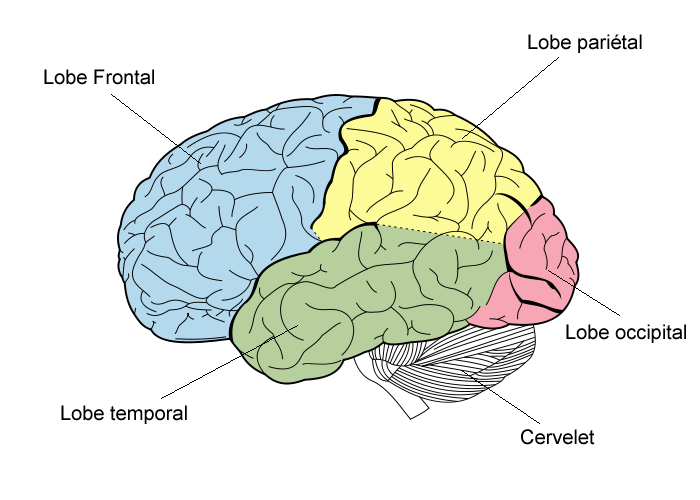
\includegraphics[width=8cm]{images/brainMap1.png}
	\caption[Représentation des différents lobes du cerveau]{Représentation des différents lobes du cerveau\\Source : http://commons.wikimedia.org/wiki/File:Lobes\_of\_the\_brain\_NL.svg?uselang=fr }
	\label{fig:brainmap2}
\end{figure}

\subsection{Lobes limbiques}
\label{Subsection: 2.Lobes limbiques}

Les lobes limbiques sont les élements du cerveau qui ne sont visibles que lorsque l'on en réalise une coupe. (Figure \ref{fig:limbique})
En voici la liste, ainsi que leurs principales fonctions : 

\begin{itemize}
	\item \textbf{Tronc cérébral}. Responsable des rythmes biologiques (respiration, rythme cardiaque, etc.).
	\smallbreak
	\item \textbf{Hippocampe}. Mémoire et navigation spatiale. 
	\smallbreak
	\item \textbf{Amygdale}. Régulation des émotions et apprentissage. 
	\smallbreak
	\item \textbf{Thalamus}. Relais et intégration des informations sensorielles (touché, vision, audition, goût).
	\smallbreak
	\item \textbf{Ganglions de la base}. Jouent un rôle dans le contrôle des mouvements. 
	\smallbreak
	\item \textbf{Hypothalamus}. Responsable de l'équilibre intérieur, c'est-à-dire les sensations de soif, de faim, la température corporelle, la sécrétion d'hormones, etc. 
	\smallbreak
	\item \textbf{Circonvolution cingulaire}. Ajuste certains paramètres corporels en fonction des émotions (pression sanguine, taille des pupilles, etc.)
	\smallbreak
	\item \textbf{Corps calleux}. Relie les deux hémisphères du cortex cérébral. 
	\smallbreak
	\item \textbf{Cervelet}. Joue un rôle essentiel dans le contrôle moteur.
\end{itemize}

\smallbreak
\begin{figure}[h]
	\centering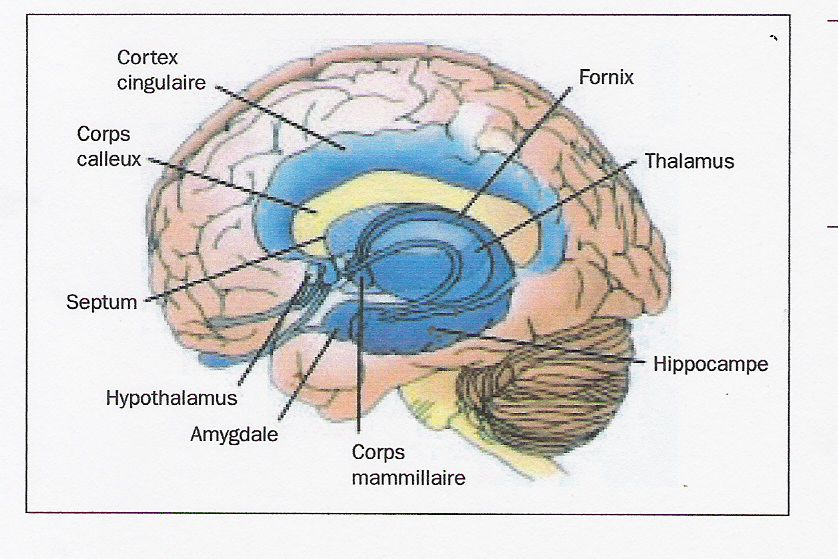
\includegraphics[width=11cm]{images/lobesLimbiques.jpg}
	\caption[Système limbique du cerveau humain.]{Système limbique du cerveau humain.\\Source : http://lucebarrault-psy.wifeo.com/article-73000-le-systeme-emotionnel.html}
	\label{fig:limbique}
\end{figure}

\section {Activité neuronale et potentiel d'action}
\label{Section: 2.Activité neuronale et potentiel d'action}

Le système nerveux est constitué de cellules nerveuses et de cellules gliales, situées entre les neurones. Chaque cellule nerveuse est composée de trois éléments : l'arbre dendritique, la synapse et le corps cellulaire (ou soma) (Figure \ref*{fig:structure d'un neurone}). Celles-ci répondent à des stimuli et envoient des informations vers d'autres neurones. L'axone est un long cylindre transmettant des impulsions électriques. Chaque dendrite est connectée aux axones ou aux dendrites d'autres neurones (environ 10 000), formant ainsi un réseau neuronal. La zone de connexion entre une dendrite et un axone est appelée la synapse. Le neurone post-synaptique reçoit alors de la part du neurone pré-synaptique une impulsion, puis la relaie à d'autres cellules nerveuses. L'activité neuronale du cerveau est en partie liée aux courants électriques échangés au niveau des synapses. Sans activité synaptique, on mesure un potentiel membranaire de -70mV au niveau du neurone, on dit qu'il est au repos. Ce potentiel membranaire change en fonction de l'activité des synapses. Si celui-ci dépasse un certain seuil, le neurone va alors émettre un potentiel d'action vers un neurone post-synaptique \cite{Saeid}.

\begin{figure}[h]
	\centering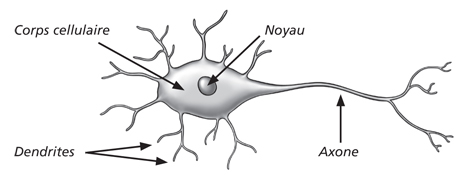
\includegraphics[width=11cm,height=4cm]{images/neurone.jpg}
	\caption[Structure d'une cellule neuronale]{Structure d'une cellule neuronale\\Source : http://www.thierrysouccar.com/bien-etre/info/comment-fonctionne-le-cerveau-386}
	\label{fig:structure d'un neurone}
\end{figure}


\section {Signaux EEG et rythmes du cerveau}
\label{Section: 2.Signaux EEG et rythmes du cerveau}

Un signal électroencéphalographique (ou signal EEG) correspond au champ électrique créé lors des échanges de courant entre les différents neurones du cerveau, au niveau des synapses. Celui-ci est mesurable au niveau de la boite crânienne grâce à des électrodes. Lors d'un EEG, on observe plusieurs signaux caractéristiques (ou ondes cérébrales). Elles correspondent à un état cognitif particulier du cerveau, i.e. l'activité physique ou intellectuelle de l'individu. Elles sont décomposées en fonction de leur domaine fréquentiel \cite{Saeid} :

\begin{itemize}
	\item \textbf{<4 Hz : Ondes Delta.}
	Elles sont généralement associées à un sommeil profond ou à certains cycles du sommeil. 
	\smallbreak
	\item \textbf{4-8 Hz : Ondes Thêta}.
	Ces ondes sont la plupart du temps liées à l'état de somnolence d'un individu, la méditation profonde, la créativité et dans un cadre plus général à tout ce qui se rapporte à l'inconscience. C'est pour cela que le changement de rythme des ondes thêta est souvent observé lorsque l'on étudie l'activité émotionnelle d'une personne.
	Ces ondes proviennent la plupart du temps de l'activité du thalamus. 
	\smallbreak
	\item \textbf{9-14 Hz : Ondes Alpha}.
	Elles caractérisent un état de conscience dans lequel un individu est dans une phase de "relaxation". Se sont les ondes les plus courantes dans le cerveau. Elles proviennent en général de la région occipitale du cortex.
	\smallbreak
	\item \textbf{15-30 Hz : Ondes Bêta}.
	Ces ondes sont liées à l'état d'éveil du cerveau, notamment lorsqu'une personne est dans un état de réflexion ou d'attention important. Ces signaux sont en général observés dans la région frontale et centrale du cortex. 
	\smallbreak
	\item \textbf{>30 Hz : Ondes Gamma}.
	Elles sont associées à certaines actions motrices du corps humain et sont généralement observées au niveau de la zone frontale du cortex. 
\end{itemize}

\smallbreak

Dans le cadre de notre projet, nous nous interesserons essentiellement aux ondes alpha et bêta.
